%%%%%%%%%%%%%%%%%%%%%%%%%%%%%%%%%%%%%%%%%%%%%%%%%%%%%%%%%%%%%%%%%%%%%%%%%%%%%%%%%%%%%%%
%%%%%%%%%%%%%%%%%%%%%%%%%%%%%%%%%%%%%%%%%%%%%%%%%%%%%%%%%%%%%%%%%%%%%%%%%%%%%%%%%%%%%%%
% 
% This top part of the document is called the 'preamble'.  Modify it with caution!
%
% The real document starts below where it says 'The main document starts here'.

%!TEX TS-program = xelatex
%!TEX encoding = UTF-8 Unicode
\documentclass[12pt]{article}

\usepackage{amssymb,amsmath,amsthm}
\usepackage[top=1in, bottom=1in, left=1.25in, right=1.25in]{geometry}
\usepackage{fancyhdr}
\usepackage{enumerate}
\usepackage{hieroglf}
\usepackage{oands}
\usepackage{pgffor, babyloniannum}
\usepackage{arevmath}
\usepackage{relsize}
\newcommand{\Bnum}[1]{{\LARGE \babyloniannum{#1}}}










% Comment the following line to use TeX's default font of Computer Modern.
\usepackage{times,txfonts}

\newtheoremstyle{homework}% name of the style to be used
  {18pt}% measure of space to leave above the theorem. E.g.: 3pt
  {12pt}% measure of space to leave below the theorem. E.g.: 3pt
  {}% name of font to use in the body of the theorem
  {}% measure of space to indent
  {\bfseries}% name of head font
  {:}% punctuation between head and body
  {2ex}% space after theorem head; " " = normal interword space
  {}% Manually specify head
\theoremstyle{homework} 

% Set up an Exercise environment and a Solution label.
\newtheorem*{exercisecore}{Exercise \@currentlabel}
\newenvironment{exercise}[1]
{\def\@currentlabel{#1}\exercisecore}
{\endexercisecore}

\newcommand{\localhead}[1]{\par\smallskip\noindent\textbf{#1}\nobreak\\}%
\newcommand\solution{\localhead{Solution:}}

%%%%%%%%%%%%%%%%%%%%%%%%%%%%%%%%%%%%%%%%%%%%%%%%%%%%%%%%%%%%%%%%%%%%%%%%
%
% Stuff for getting the name/document date/title across the header
\makeatletter
\RequirePackage{fancyhdr}
\pagestyle{fancy}
\fancyfoot[C]{\ifnum \value{page} > 1\relax\thepage\fi}
\fancyhead[L]{\ifx\@doclabel\@empty\else\@doclabel\fi}
\fancyhead[C]{\ifx\@docdate\@empty\else\@docdate\fi}
\fancyhead[R]{\ifx\@docauthor\@empty\else\@docauthor\fi}
\headheight 15pt

\def\doclabel#1{\gdef\@doclabel{#1}}
\doclabel{Use {\tt\textbackslash doclabel\{MY LABEL\}}.}
\def\docdate#1{\gdef\@docdate{#1}}
\docdate{Use {\tt\textbackslash docdate\{MY DATE\}}.}
\def\docauthor#1{\gdef\@docauthor{#1}}
\docauthor{Use {\tt\textbackslash docauthor\{MY NAME\}}.}
\makeatother

% Shortcuts for blackboard bold number sets (reals, integers, etc.)
\newcommand{\Reals}{\ensuremath{\mathbb R}}
\newcommand{\IRats}{\ensuremath{\mathbb I}}
\newcommand{\Nats}{\ensuremath{\mathbb N}}
\newcommand{\Ints}{\ensuremath{\mathbb Z}}
\newcommand{\Rats}{\ensuremath{\mathbb Q}}
\newcommand{\Cplx}{\ensuremath{\mathbb C}}
%% Some equivalents that some people may prefer.
\let\RR\Reals
\let\NN\Nats
\let\II\Ints
\let\CC\Cplx


\doclabel{Math F316}
\docauthor{Stefano Fochesatto}
\docdate{\today}% DATE READING SENTENCES ARE DUE GOES HERE


%%%% Main document starts here.

\begin{document}

\section*{Section 1.2}

\begin{exercise}{1} Express each of the given numbers in Egyptian hieroglyphics.\\
    \begin{enumerate}
        \item 1,492 
        \solution
        
        \cartouche{\pmglyph{\Hthousand \Hhundred \Hhundred \Hhundred \Hhundred \Hten \Hten \Hten \Hten \Hten \Hten \Hten \Hten
        \Hten \Hone \Hone}}

        \item 12,321
        \solution
        
        \cartouche{ \pmglyph{\HXthousand \Hthousand \Hthousand \Hhundred \Hhundred \Hhundred \Hten \Hten \Hone}}

    \end{enumerate}
\end{exercise}


\begin{exercise}{2} Write the following egyptian number in our system.\\

    \cartouche{ \pmglyph{\Hone-\Hone-\Hone-\Hone-\Hone-\Hone-\Hone-\Hone-\Hten-\Hten-\Hten-\Hten-\Hhundred-\Hhundred-\Hhundred-\Hhundred-\Hhundred-\Hhundred}}
    \solution

    648
\end{exercise}


\begin{exercise}{3} Perform the indicated operations and express the answers in hieroglyphics.\\
    \begin{enumerate}
        \item  Addition\\
        
        \begin{center}
        \cartouche{ \pmglyph{\Hone-\Hone-\Hone-\Hone-\Hone-\Hone-\Hone-\Hthousand-\HXthousand-\HXthousand-\HXthousand-\HXthousand-\HXthousand-\HXthousand}}\\
        \cartouche{ \pmglyph{\Hone-\Hone-\Hone-\Hone-\Hone-\Hten-\Hhundred-\Hhundred-\HXthousand-\HXthousand-\HXthousand-\HXthousand-\HXthousand}}
        \end{center}
        \begin{center}
            \cartouche{ \pmglyph{\Hone-\Hone-\Hone-\Hone-\Hone-\Hone-\Hone-\Hone-\Hone-\Hone-\Hone-\Hone-\Hten-\Hhundred-\Hhundred-\Hthousand-\HXthousand-\HXthousand-\HXthousand-\HXthousand-\HXthousand-\HXthousand-\HXthousand-\HXthousand-\HXthousand-\HXthousand-\HXthousand}}
        \end{center}
        \begin{center}
            \cartouche{ \pmglyph{\Hone-\Hone-\Hten-\Hten-\Hhundred-\Hhundred-\Hthousand-\HXthousand-\HCthousand}}
        \end{center}

        \item Subtract\\
        \begin{center}
            \cartouche{ \pmglyph{\Hone-\Hone-\Hten-\Hten-\Hten-\Hthousand}}\\
            \cartouche{ \pmglyph{\Hone-\Hone-\Hone-\Hone-\Hten-\Hten-\Hten-\Hten-\Hhundred-\Hhundred-\Hhundred}}
            \end{center}
            \begin{center}
                \cartouche{ \pmglyph{\Hone-\Hone-\Hone-\Hone-\Hone-\Hone-\Hone-\Hone-\Hten-\Hten-\Hten-\Hten-\Hten-\Hten-\Hten-\Hten-\Hhundred-\Hhundred-\Hhundred-\Hhundred-\Hhundred-\Hhundred}}
            \end{center}
    \end{enumerate}
\end{exercise}



\begin{exercise}{5} Write the Ionian Greek numerals corresponding to 396.

    \solution tau koppa digamma
\end{exercise}


\begin{exercise}{11} Write the corresponding Roman Numerals
    \begin{enumerate}
        \item 1,492
        \solution $MCDXCII$
        
        \item 3,040,279
        \solution $\overline{MMMXL}CCLXXIX$
        \end{enumerate}
\end{exercise}

\begin{exercise}{12} Convert the following Roman Numeral, $MDCCXLVIII$
    \solution 
    \begin{equation*}
    1000 + 700 + 40 + 8 = 1748
    \end{equation*}
    
\end{exercise}




\section*{Section 1.3}

\begin{exercise}{1} Express the following in Babylonian cuneiform notation, 12,345.
\solution
We must convert 12345 to base 60, then use the cuneiform notation to represent our base 60 
representation. Converting we get, 
\begin{equation*}
    123456 \div 3600 \approx 3.
\end{equation*}
Dividing the remainder by 60 we get, 
\begin{equation*}
    (12345 - (3600*3))\div 60 \approx 25.
\end{equation*}
Calculating the final remainder,
\begin{equation*}
    (1545 - (60*25)) = 45
\end{equation*}
Thus in base 60 we get that $12345 \to (3,25,45)_{60}$. Applying cuneiform notation,
\begin{center}
    \Bnum{12345}    
\end{center}
\end{exercise}


\begin{exercise}{2} Translate the following number into our system,
    \begin{center}
        \Bnum{52806}
    \end{center}
    \solution Rewriting the cuneiform notation, we get that $(14, 40, 6)_{60}$. Multiplying by the 
    base 60 digits, we get that,
    \begin{equation*}
        (3600*14)+(60*40)+(6) = 52806
    \end{equation*} 

    
\end{exercise}


\begin{exercise}{3} Express the fractions $\frac{1}{6}$, $\frac{1}{40}$, and $\frac{5}{12}$ in sexagesimal notation. \\
\solution For the fraction $\frac{1}{6}$ we can already see that, 
\begin{equation*}
    \frac{1}{6} = \frac{10}{60}.
\end{equation*}
Therefore we get that,
\begin{equation*}
    \frac{1}{6} =  ;\Bnum{10}
\end{equation*}

For the fraction $\frac{1}{40}$ we can see that $\frac{1}{60}$ fits into $\frac{1}{40}$ with a remainder of
$\frac{1}{120}$. Since, 
\begin{equation*}
    \frac{1}{120} = \frac{30}{3600}.
\end{equation*}
Therefore we get the following,
\begin{equation*}
 \frac{1}{40} =;\Bnum{1},\Bnum{30}    
\end{equation*}

For the function $\frac{5}{12}$ we can simply see that for the function,
\begin{equation*}
    \frac{1}{12} = \frac{5}{60}.
\end{equation*}
Applying addition to get $\frac{5}{12}$,
\begin{equation*}
    \frac{5}{12} = ;\Bnum{25}
\end{equation*}

\end{exercise}


\begin{exercise}{4} Convert $12;3,45$ from sexagesimal notation into our system.
    \solution Applying our algorithm to convert we get that, 
    \begin{equation*}
        (12*1)+(3*\frac{1}{60})+(45*\frac{1}{3600}) = 12 + \frac{1}{20} + \frac{1}{80}.
    \end{equation*}
    Simplifying we get that, 
    \begin{equation*}
        12;3,45 = 12 + \frac{1}{16} = \frac{193}{16}
    \end{equation*}
\end{exercise}



\begin{exercise}{6} Write 1,492 in Chinese counting-rod numerals
    \solution 
    \begin{center}
        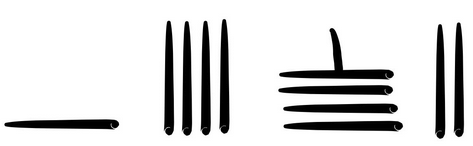
\includegraphics[width = .33\textwidth]{chin.png}        
    \end{center}
    
\end{exercise}

\begin{exercise}{7} Convert the following Chinese counting-rod numerals into our system,
    \begin{center}
        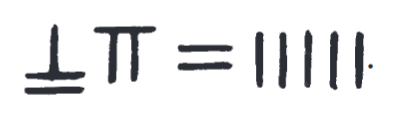
\includegraphics[width = .33\textwidth]{chin2.png}        
    \end{center}
    
    \solution Using the conversion table we get the following, 7,725
    
\end{exercise}



\begin{exercise}{13} Write the Mayan Priest numerals corresponding to 1492,
    \solution First we divide 1492 by 360 and get, 4 with a remainder of 52. 
    Then we divide 52 by 20 to get 2 with a remainder of 12. Therefore the following is the 
    Mayan Priest representation of 1492,
    \begin{center}
        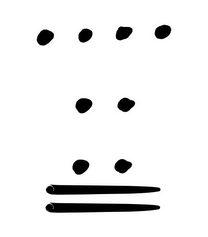
\includegraphics[width = .15\textwidth]{Maya.png}        
    \end{center}
    
\end{exercise}

\begin{exercise}{14} Convert the following Mayan Priest numeral into our system, 
    \begin{center}
        
\includegraphics[width = .15\textwidth]{Maya2.png}        
    \end{center}
    \solution Multiplying by base for each digit we get that,
    \begin{equation*}
        (13*7200)+(0*360)+(5*20)+(7) = 93707.
    \end{equation*}
\end{exercise}



\section*{Section 2.3}

\begin{exercise}{1} Use the egyptian method of doubling to find $18*25$
        \solution Taking the smaller term in the product and doubling it until we find a 
        left hand exponent of 2 that is larger than 25, 
        \begin{align*}
            1 &|18\\
            2 &|36\\
            4 &|27\\
            8 &|144\\
            16 &|288\\
            32 &|576
        \end{align*}
        Note that $16+8+1 = 25$ thus we get that the product $18*25 = 288+144+18 = 450$

    
\end{exercise}



\begin{exercise}{2} Find, in Egyptian fashion the following quotients. \\
    \begin{enumerate}
        \item $184 \div 8$
        \solution Again taking the smaller term from the quotient and doubling it to create a table,
        \begin{align*}
            1 &|8\\
            2 &|16\\
            4 &|32\\
            8 &|64\\
            16 &|128
        \end{align*}
        Now we need to see which terms on the right hand side of the table sum to 184. Note that,
        \begin{equation*}
            128 + 32 + 16 + 8 = 184
        \end{equation*}
        Summing the corresponding terms on the left hand side we arrive at the answer, 
        \begin{equation*}
            16 + 4 + 2 + 1 = 23
        \end{equation*}
    
    \item $19 \div 8$
    \solution Taking the smaller term from the quotient and constructing the table again. This time we will need
    to divide by 2 as well since 8 is not a divisor of 19.
    \begin{align*}
        \overline{8} &|1\\ 
        \overline{4} &|2\\ 
        \overline{2} &|4\\ 
        1 &|8\\
        2 &|16
    \end{align*}
    Summing again we can see that, $16 + 2 + 1 = 19$. Thus summing on the left hand side we get that, 
    \begin{equation*}
        2 + \overline{4} + \overline{8}
    \end{equation*}
\end{enumerate}
    
\end{exercise}
    
    \begin{exercise}{3} Use the Egyptian method of multiplication to calculate $(11 + \overline{2} + \overline{8})37$.
        \solution In this case we will construct the table again with $(11 + \overline{2} + \overline{8})$
        \begin{align*}
            1 &| 11 + \overline{2} + \overline{8}\\ 
            2 &| 23 + \overline{4}\\ 
            4 &| 46 + \overline{2}\\ 
            8 &| 93\\
            16 &| 186 \\
            32 &| 372
        \end{align*}
        Note that $32 + 4 + 1 = 37$, therefore summing the corresponding right hand values we get, 
        \begin{equation*}
            372 + 46 + \overline{2} + 11 + \overline{2} + \overline{8} = 430 + \overline{8}
        \end{equation*}
    \end{exercise}
    


    \begin{exercise}{5} Problem 309 of the Rhind Papyrus asks the reader to find a quantity such that $\overline{\overline{3}} + \overline{10}$
        of it will make $10$. Do this as the Egyptians would have sone, first by confirming that, 
        \begin{equation*}
            13(\overline{\overline{3}} + \overline{10}) = 9 + \frac{29}{30}
        \end{equation*}
        Then determine by what amount $\overline{\overline{3}} + \overline{10}$ should be multiplied to give $\overline{30}$.
        \solution The question suggests that when using the method of false position we should let $x = 13$. Therefore finding the product of $13(\overline{\overline{3}} + \overline{10})$
        by a table, 
        \begin{align*}
            1 &|\overline{\overline{3}} + \overline{10}\\
            2 &|1 + \overline{3} + \overline{5}\\
            4 &|2 + \overline{\overline{3}} + \overline{5} + \overline{6} + \overline{30}\\
            8 &|5 + \overline{\overline{3}} + \overline{5} + \overline{6} + \overline{15} + \overline{30}
        \end{align*}
       
        Summing to 13 on the left hand side we see that, $13 = 8 + 4 + 1$. Summing the corresponding left hand values, we find that,
        \begin{equation*}
            \overline{\overline{3}} + \overline{10} + 2 + \overline{\overline{3}} + \overline{5} + \overline{6} + \overline{30} + 5 + \overline{\overline{3}} + \overline{5} + \overline{6} + \overline{15} + \overline{30}
        \end{equation*}
        We get the following in Egyptian form, 
        \begin{equation*}
            9 + \overline{3} + \overline{5} + \overline{6} + \overline{10} + \overline{15} + \overline{16}+ \overline{30} + \overline{240} 
         \end{equation*}
         Expanding and adding in our system we do find that,
         \begin{equation*}
            \overline{3} + \overline{5} + \overline{6} + \overline{10} + \overline{15} + \overline{16}+ \overline{30} + \overline{240}  = \frac{29}{30}.
         \end{equation*}
         Solving for the factor that we need to multiply $(\overline{\overline{3}} + \overline{10})$ using our system, 
         \begin{align*}
             x(\frac{2}{3}+ \frac{1}{10}) &= \frac{1}{30}\\
             \frac{23x}{30} &= \frac{1}{30}\\
             x &= \frac{1}{23}
         \end{align*}
         Thus the quantity is $13 + \overline{23}$.
    \end{exercise}


    \begin{exercise}{19} Divide 9 loaves equally among 10 men, solve by false position.
        \solution First suppose that the problem would be written in this form 
        \begin{equation*}
            10x = 9.
        \end{equation*}
        Lets suppose that the quantity $x = \overline{10}$, this gives us that
        \begin{equation*}
            10*\overline{10} = 1.
        \end{equation*} 
        To make $1$ into $9$ we simply multiply the quantity by $9$. Therefore we must solve $\overline{10}*9$. With a table we get that,
        \begin{align*}
            1 &| \overline{10}\\
            2 &| \overline{5}\\
            4 &| \overline{5} + \overline{6} + \overline{30}\\
            8 &| \overline{3} + \overline{5} + \overline{6} + \overline{15} + \overline{30}
        \end{align*}
        Note that $8 + 1 = 9$ and thus summing the corresponding right hand values gives us our answer, 
        \begin{equation*}
            x = \overline{3} + \overline{5} + \overline{6} + \overline{10} + \overline{15} + \overline{30} = (\frac{9}{10})
        \end{equation*}

    \end{exercise}
    
    





    \begin{exercise}{20} What quantity and it's $\frac{1}{5}$ added together become 21.
        \solution Consider this problem written in our notation, 
        \begin{equation*}
            x + \frac{x}{5} = 21.
        \end{equation*} 
        Using the method of false position, lets suppose that $x = 5$, therefore we get the following, 
        \begin{equation*}
            5 + 1 = 6.
        \end{equation*}
        Note that 6 must be multiplied by $\frac{21}{6} = 3 + \overline{2}$ to obtain the right answer and therefore we know that the 
        quantity is the product $5*(3 + \overline{2})$. We could use doubling to find this product but I think an egyptian student could see that, 
        \begin{equation*}
        5*(3 + \overline{2}) = 17 + \overline{2}    
        \end{equation*}
        Substituting back into the original problem with $x = 17 + \overline{2}$ we can see that, 
        \begin{equation*}
            (17 + \overline{2}) + \frac{5*(3 + \overline{2})}{5} = 20 + \overline{2} + \overline{2} = 21.
        \end{equation*}


    \end{exercise}






\end{document}
